\documentclass[a4paper,12pt]{article}

% --- LANGUAGE & FONT ---
\usepackage{vntex}
\usepackage[english]{babel}
\usepackage{amsmath, amssymb}

% --- PAGE & TEXT LAYOUT ---
\usepackage{a4wide}
\usepackage{geometry}
\geometry{a4paper, left=2cm, right=2cm, top=2.5cm, bottom=4.2cm, footskip=12mm}
\usepackage{setspace}
\usepackage{multicol}
\usepackage{enumitem}

% --- GRAPHICS & TABLES ---
\usepackage{graphicx}
\usepackage{epsfig}
\usepackage{svg}
\usepackage{tikz}
\usetikzlibrary{arrows,snakes,backgrounds,positioning,shapes,calc,fit}
\usepackage{booktabs}
\usepackage{multirow}
\usepackage{tabularx}
\usepackage{makecell}
\usepackage{array}
\usepackage[skip=5pt]{caption}
\usepackage{placeins}
\usepackage{float}       % added: the template uses [H]
\usepackage{longtable}   % added: long tables across pages

% --- COLOURS & CODE ---
\usepackage{color}
\usepackage{xcolor}
\usepackage{colortbl}    % added: coloured table rows
\usepackage{minted}
\usepackage{listings}
\usepackage{algorithm}
\usepackage{algpseudocode}
\usepackage[framemethod=tikz]{mdframed}

% --- HEADER & FOOTER ---
\usepackage{fancyhdr}
\usepackage{lastpage}

% --- HYPERREF (always load last) ---
\usepackage{hyperref}
\hypersetup{urlcolor=blue,linkcolor=black,citecolor=black,colorlinks=true}

% ================= COLOURS =================
\setlength{\columnseprule}{1pt}
\def\columnseprulecolor{\color{black}}
\definecolor{p1}{RGB}{52,101,164}
\definecolor{p2}{RGB}{78,154,6}
\definecolor{p3}{RGB}{204,0,0}
\definecolor{p4}{RGB}{117,80,123}
\definecolor{p5}{RGB}{193,125,17}
\definecolor{p6}{RGB}{32,128,128}
\definecolor{p7}{RGB}{90,90,90}
\definecolor{p8}{RGB}{170,60,120}

% ================= HEADER/FOOTER =================
\everymath{\color{blue}}
\setlength{\headheight}{40pt}
\pagestyle{fancy}
\fancyhead{}
\fancyhead[L]{
 \begin{tabular}{rl}
    \begin{picture}(25,15)(0,0)
    \put(0,-8){
\includegraphics[width=8mm, height=8mm]{hcmut.png}}
   \end{picture}&
    \begin{tabular}{l}
        \textbf{\ttfamily Ho Chi Minh City University of Technology - VNU-HCM}\\
        \textbf{\ttfamily Faculty of Computer Science and Engineering}
    \end{tabular}
 \end{tabular}
}
\fancyhead[R]{}
\fancyfoot{}
\fancyfoot[L]{\scriptsize \ttfamily \textcolor{blue}{Builders Buildathon 2026 - P4 Blast Radius \\ Team HCMUT TMT, November 2026}}
\fancyfoot[R]{\scriptsize \ttfamily Page {\thepage}/\pageref{LastPage}}
\renewcommand{\headrulewidth}{0.3pt}
\renewcommand{\footrulewidth}{0.3pt}

\setcounter{secnumdepth}{4}
\setcounter{tocdepth}{3}

% ================= COLOURED BOXES =================
% \partbox{color}{title}{content}: short box, no page break
\newcommand{\partbox}[3]{%
\begin{mdframed}[nobreak=true,linecolor=#1,linewidth=1.2pt,topline=false,rightline=false,bottomline=false,leftmargin=0pt,rightmargin=0pt,innerleftmargin=10pt,backgroundcolor=#1!6]
\textbf{\color{#1}#2}\par\smallskip #3
\end{mdframed}}
% \longbox{color}{title}{content}: long box, may break across pages
\newcommand{\longbox}[3]{%
\begin{mdframed}[linecolor=#1,linewidth=1.2pt,topline=false,rightline=false,bottomline=false,leftmargin=0pt,rightmargin=0pt,innerleftmargin=10pt,backgroundcolor=#1!6]
\textbf{\color{#1}#2}\par\smallskip #3
\end{mdframed}}
% \metabox{color}{workload}{prerequisites}{foundation for}{people}
\newcommand{\metabox}[5]{%
\begin{mdframed}[nobreak=true,linecolor=#1,linewidth=1pt,leftmargin=0pt,rightmargin=0pt,backgroundcolor=#1!15]
\textbf{Workload:} #2\par
\textbf{Prerequisites:} #3\par
\textbf{Foundation for:} #4\par
\textbf{People:} #5
\end{mdframed}}

% ================= HELPER MACROS (added for this report) =================
% \trial{...}: trial-run figure, not an official result
\newcommand{\trial}[1]{\textcolor{p5}{\textbf{[trial run]}~#1}}
% \src{...}: source of a figure
\newcommand{\src}[1]{{\footnotesize\textcolor{p7}{(source: #1)}}}
\newcommand{\fn}[1]{\texttt{\detokenize{#1}}}
\newcolumntype{L}[1]{>{\raggedright\arraybackslash}p{#1}}
\newcolumntype{C}[1]{>{\centering\arraybackslash}p{#1}}
\newcolumntype{Y}{>{\raggedright\arraybackslash}X}
\setlist{itemsep=1pt,topsep=2pt}
\renewcommand{\arraystretch}{1.15}

\begin{document}

\begin{titlepage}
\begin{center}
\Large Vietnam National University Ho Chi Minh City \\
\Large Ho Chi Minh City University of Technology \\
\Large Faculty of Computer Science and Engineering
\end{center}

\vspace{1cm}
\begin{center}

\includegraphics[width=4cm]{hcmut.png}
\end{center}
\vspace{1cm}

\begin{center}
\begin{tabular}{c}
    \textbf{\Large BUILDERS BUILDATHON 2026} \\[0.2cm]
    \textbf{\Large (Problem 4)} \\
    ~~\\
    \hline
    \\
    \multicolumn{1}{l}{\textbf{{\Large Problem overview}}}\\
    \\
    \textbf{{\LARGE RWX -- Blast Radius}}\\[0.2cm]
    {\large Choosing which tests to run for each change to sqlglot}\\
    \\
    \hline
\end{tabular}
\end{center}

\vspace{0.5cm}

\begin{table}[h]
\centering
\begin{tabular}{rrl}
\hspace{2cm} & Track: & RWX - Blast Radius \\
& Team: & HCMUT TMT\\
& Student: & Dang Minh Triet - 2510249 \\
& Deadline: & 23:00 Sunday 22/11/2026 (GMT+7) \\
\end{tabular}
\end{table}

\vfill
\begin{center}
{\footnotesize Ho Chi Minh City, November 2026}
\end{center}
\end{titlepage}

\thispagestyle{fancy}
\newpage
\tableofcontents
\newpage

\sloppy

\section{Overview}

\subsection{General information}
\begin{table}[H]
\centering\small
\begin{tabularx}{\textwidth}{L{4.3cm}Y}
\toprule
\textbf{Item} & \textbf{Details} \\
\midrule
Track & RWX -- Blast Radius (sponsor RWX, \$5{,}000 prize, 116 teams on the practice board at the time of the screenshot) \\
Problem & Each commit is a patch to sqlglot at commit \fn{eb11aec4be8cb2122afe713a4816662c3f0fb2fa}. The program prints which tests to run and how to split them across up to 8 workers \\
Deadline & \textbf{23:00 Sunday 22/11/2026 (GMT+7)}. At the time of writing (Sat 21/11, around 11:10) about 36 hours remain \\
Submission limit & Once an hour to start (organisers raise it if the queue stays short); the submit panel showed ``1 of 1 left this hour'' \\
How to submit & Public GitHub repo, \fn{Dockerfile} at the root, plus a commit hash. Repo at most 20 MB \\
Build & Network on, 4 cores, 8 GB RAM, 10 minutes. Downloads only from PyPI, npm, Docker Hub, GitHub releases at a fixed tag, and sqlglot at the pinned commit \\
Run & No network, 2 cores, 4 GB, \textbf{3 minutes for the whole batch} (4.5 minutes in the final, about 1.5 times as many commits), user \fn{nobody}, \fn{HOME=/tmp}, read-only disk, \fn{/tmp} 64 MB, at most 256 processes, stdout at most 2 MB \\
Final & The chosen commit (by default the best practice submission) is scored on unseen commits, \emph{including kinds of change not in practice}. At least the top 5 are scored again 5 times on an idle machine, and the median counts \\
\bottomrule
\end{tabularx}
\caption{General information for P4 \src{track page, README.md, SCORING.md}}
\end{table}

\subsection{Scoring and how it is graded}
P4 has a single criterion, \textbf{graded fully automatically} by the scorer (same rules as \fn{score.py} in the kit). There is no AI grading. There is one \textbf{human} element: the organisers state ``Top entries are read'', meaning people read the code of the leading teams to check the rules (no patch $\rightarrow$ test lookup tables, no code sharing between teams).

\begin{table}[H]
\centering\small
\begin{tabularx}{\textwidth}{L{3.6cm}Y C{1.9cm}C{1.4cm}}
\toprule
\textbf{Component} & \textbf{Definition} & \textbf{Graded by} & \textbf{Part} \\
\midrule
Cost of one commit & Largest worker load (sum of recorded seconds of the tests in that worker) $+\;2$ s $\times$ number of workers. Running nothing costs 0 & auto & 4.3, 4.4 \\
Miss penalty & $+300$ s for each commit where at least one failing test is in no worker & auto & 4.2, 4.5 \\
CPU & Total CPU (user + system) of every process in the container, from start to exit & auto & 4.1, 4.3 \\
Submission score & The image runs 3 times; the middle total counts, rounded to 0.1 s: $\lfloor(\mu s+50000)/100000\rfloor/10$ & auto & 4.6 \\
Rule check & Top entries' code is read; same repo/commit as another team disqualifies the later one & human & 4.5 \\
\bottomrule
\end{tabularx}
\caption{P4 rubric \src{SCORING.md, track page}}
\end{table}

\[
\text{total} \;=\; \sum_{\text{commit}}\Big(\max_{w}\sum_{t\in w} d_t \;+\; 2\cdot|W|\Big) \;+\; 300\cdot \#\text{misses} \;+\; \text{CPU},
\]
where $d_t=\mathrm{round}(1000\cdot\text{seconds}_t)$ ms.

\begin{table}[H]
\centering\small
\begin{tabular}{lrl}
\toprule
\textbf{Practice board (screenshot 21/11)} & \textbf{Score} & \textbf{Note} \\
\midrule
Rank 1 (SophiaOmri) & 153.7 s & \\
Rank 2 (fortnite pirate token) & 156.8 s & \\
Starter baseline & 1614.1 s & Every test, split over 3 workers \\
Teams & 116 & \\
\bottomrule
\end{tabular}
\caption{Practice leaderboard snapshot (for orientation only; the practice board carries no prize)}
\end{table}

\begin{mdframed}[linecolor=orange,linewidth=1pt,backgroundcolor=orange!8]
\textbf{Inference (not confirmed):} On the 30 sample commits the starter costs 40.349 s/commit (see the trial table in 4.6). $1614.1/40.349 \approx 40.0$, so the practice set most likely has about \textbf{40 commits}, and the final about 60. The leading team spends about 3.8 s/commit, close to the ``oracle'' level (knowing in advance which tests fail) of 4.5 s/commit on the sample set. In other words the top teams select tests almost perfectly.
\end{mdframed}

\subsection{Sources and conventions for figures}
\begin{itemize}
  \item \textbf{Primary sources:} the track page (screenshot) and \fn{SCORING.md}. The repo has no forum Q\&A yet; when organiser answers exist they take precedence.
  \item \textbf{For reference:} \fn{README.md}, \fn{selector.py}, \fn{score.py}, \fn{Makefile}, \fn{Dockerfile}, \fn{requirements.lock} and the 30 sample commits in \fn{p4_RWX/starter_files/blast-radius-sample/}.
  \item Figures marked \trial{} come from running \fn{score.py} on the sample set myself; they are \emph{not official results}. The official board also adds CPU and takes the median of 3 runs.
\end{itemize}

\subsection{Dependency diagram}
\begin{center}
\begin{tikzpicture}[
  box/.style={draw,rounded corners,thick,text width=3.3cm,minimum height=1.2cm,align=center,font=\small},
  ext/.style={draw,dashed,rounded corners,text width=3.6cm,minimum height=1cm,align=center,font=\small,fill=gray!8},
  arr/.style={->,thick,>=stealth},
  lab/.style={font=\scriptsize,fill=white,inner sep=1pt}]
  \node[ext] (c) at (0,2.6) {\textbf{Shared}: public repo, Docker (shared with P1, P2)};
  \node[box,draw=p1,fill=p1!10] (a) at (0,0) {\textbf{4.1} Environment and tooling};
  \node[box,draw=p2,fill=p2!10] (b) at (5.4,0) {\textbf{4.2} Static maps: coverage, fixtures, imports};
  \node[box,draw=p3,fill=p3!10] (d) at (10.8,0) {\textbf{4.3} Patch analysis, test selection};
  \node[box,draw=p4,fill=p4!10] (e) at (5.4,-2.8) {\textbf{4.4} Optimal worker split};
  \node[box,draw=p5,fill=p5!10] (f) at (10.8,-2.8) {\textbf{4.5} Safety rules (recall)};
  \node[box,draw=p6,fill=p6!10] (g) at (10.8,-5.6) {\textbf{4.6} Evaluate, submit, pick final};
  \draw[arr] (c) -- (a);
  \draw[arr] (a) -- node[lab,above=2pt]{reference env} (b);
  \draw[arr] (b) -- node[lab,above=2pt]{maps} (d);
  \draw[arr] (a) |- (e);
  \draw[arr] (d) -- node[lab,right=2pt]{test set} (f);
  \draw[arr] (b) -- node[lab,sloped,above=2pt]{import map} (f);
  \draw[arr] (e) |- (g);
  \draw[arr] (f) -- (g);
\end{tikzpicture}
\end{center}
P4 does not depend on the results of P1, P2 or P3. The only shared pieces are infrastructure (a public GitHub repo with a root \fn{Dockerfile}, linux/amd64 builds) and one person's time budget.

\subsection{Repo status}

\begin{table}[H]
\centering\small
\begin{tabularx}{\textwidth}{L{4.2cm}Y}
\toprule
\textbf{Item} & \textbf{Status (read on 21/11, around 11:10)} \\
\midrule
Main repo & \fn{martin-danggg/HCMUT_TMT_Builders_BUILDATHON}, branch \fn{main}, remote \fn{origin} over SSH \\
Latest commit & \fn{55687de} ``Initial commit'', 21/11/2026 10:41:21 +0700, author Triet Dang. This is the only commit \\
Committed files & Only \fn{README.md} (31 bytes, a one-line title) \\
Not committed (untracked) & \fn{p1_Builders/} (2.9 MB), \fn{p2_Databricks/} (5.7 MB), \fn{p3_Machina/} (48 KB), \fn{p4_RWX/} (404 KB): all of it is starter files from the organisers; no solution code yet \\
\fn{reports/} folder & Holds this overview (Vietnamese and English, not committed) \\
Main repo \fn{.gitignore} & Ignores the 3 \fn{submission/} folders (separate repos) and \fn{p3_Machina/submission/} (P3 data must stay private) \\
Separate submission repos (created on GitHub, public) & P1: \fn{martin-danggg/hcmut-tmt-p1-mech-royale} $\rightarrow$ \fn{p1_Builders/submission/}\allowbreak\fn{hcmut-tmt-p1-mech-royale/} (commit \fn{f4e1861})\newline P2: \fn{martin-danggg/hcmut-tmt-p2-shopping-sessions} $\rightarrow$ \fn{p2_Databricks/submission/}\allowbreak\fn{hcmut-tmt-p2-shopping-sessions/} (commit \fn{21cd7e4})\newline P4: \fn{martin-danggg/hcmut-tmt-p4-blast-radius} $\rightarrow$ \fn{p4_RWX/submission/}\allowbreak\fn{hcmut-tmt-p4-blast-radius/} (commit \fn{2a682dc})\newline The starter skeleton is cloned, committed as ``Setup: add requirements'' and pushed to \fn{main} by \fn{tools/setup_submissions.sh} \\
\bottomrule
\end{tabularx}
\caption{Status of the main repo, shared by all 4 problems}
\end{table}

\begin{mdframed}[linecolor=orange,linewidth=1pt,backgroundcolor=orange!8]
\textbf{Submitting through separate repos (decided):} P1, P2 and P4 all require \emph{a public GitHub repository with the \fn{Dockerfile} at the root} of the submitted commit. The main repo is a monorepo (p1--p4 in subfolders), so \textbf{the main repo is never submitted}. Each track has its own public repo, kept locally in \fn{pX_.../submission/hcmut-tmt-pX-.../}; each of those folders is an independent git repo with its own remote, and the main repo ignores them via \fn{.gitignore}. To submit: paste the track repo's link (e.g. \fn{https://github.com/martin-danggg/hcmut-tmt-p4-blast-radius}) into \emph{Public GitHub repository}; leave \emph{Commit} empty to use the newest commit on \fn{main}. Keep the repo public, with every submitted commit, until results are published. P3 needs no GitHub (it is submitted through the team's \fn{gs://} folder).
\end{mdframed}


\begin{table}[H]
\centering\small
\begin{tabularx}{\textwidth}{L{5.2cm}C{1.9cm}Y}
\toprule
\textbf{P4 component} & \textbf{Present?} & \textbf{Note} \\
\midrule
Starter kit (\fn{selector.py}, \fn{score.py}, \fn{Makefile}, \fn{Dockerfile}) & Yes & Organisers' original, both the \fn{.tar.gz} and the unpacked copy \\
30 sample commits + \fn{tests.json} + \fn{answers.json} & Yes & 1620 numbered tests, 1 skipped \\
sqlglot checkout at \fn{eb11aec} & No & Needed for 4.2 (done offline, not committed) \\
Coverage / fixture / import maps & No & Output of 4.2 \\
New selector, worker split & No & Output of 4.3--4.5 \\
Separate submission repo \fn{hcmut-tmt-p4-blast-radius} & Yes & \fn{p4_RWX/submission/}\allowbreak\fn{hcmut-tmt-p4-blast-radius/}: the whole kit (Dockerfile, \fn{selector.py}, \fn{score.py}, \fn{Makefile}, \fn{sample/}); commit ``Setup: add requirements'' \\
\bottomrule
\end{tabularx}
\caption{What P4 already has and what is missing}
\end{table}

\subsection{Assignments and schedule}
Working alone, so the ``reviewer'' column does not apply. Instead of review, every change must pass \fn{make sample} (score and misses) before it is submitted.

\begin{table}[H]
\centering\small
\begin{tabularx}{\textwidth}{C{1cm}L{2.6cm}YC{1.6cm}}
\toprule
\textbf{Part} & \textbf{Owner} & \textbf{Task} & \textbf{Review} \\
\midrule
4.1 & Dang Minh Triet & Submission repo, environment identical to labelling, \fn{make sample} working & -- \\
4.2 & Dang Minh Triet & Per-test coverage map, fixture map, import map & -- \\
4.3 & Dang Minh Triet & Read patches, map changed lines to tests & -- \\
4.4 & Dang Minh Triet & Choose the worker count and split tests & -- \\
4.5 & Dang Minh Triet & Fallback rules for unusual cases & -- \\
4.6 & Dang Minh Triet & Compare versions, submit, pick the final & -- \\
\bottomrule
\end{tabularx}
\caption{P4 assignments}
\end{table}

There are no ``weeks'' or separate ``tag deadlines'': the only deadline is 23:00 Sunday 22/11, so the schedule is split into time blocks. Suggestion: tag the final submitted commit \fn{p4-final} in the 22:00--22:45 block so it is easy to trace. P4 gets 5.5 hours out of about 25 working hours (22\%).

\begin{center}\small
\begin{longtable}{L{1.8cm}L{2.1cm}C{1.3cm}L{10.1cm}}
\toprule \textbf{Day} & \textbf{Time} & \textbf{Track} & \textbf{Task} \\ \midrule\endhead
Sat 21/11 & 11:15--12:00 & Shared & Create 3 separate public repos for P1, P2, P4 (Dockerfile at the root); check Docker/WSL2; P3: fetch the manifest, run \fn{get-input.sh --limit 100} \\
\rowcolor{p4!15} & 12:00--15:30 & P4 & 4.1 environment + 4.2 coverage map at the pinned commit; 4.3--4.4 selector v1; \fn{make sample}; first submission \\
 & 15:30--18:00 & P1 & 1.1 infrastructure + 1.2 map + 1.3 movement/zone; submit bot v1 \\
 & 18:00--19:00 & -- & Break \\
 & 19:00--22:30 & P2 & 2.1--2.7 correct version: 36/36 fixtures, \fn{check-dev} MATCH; first submission \\
 & 22:30--23:30 & P3 & 3.1 survey 100 sample files; start the full corpus download in the background overnight \\
 & 23:30--00:30 & P1 & 1.4 combat v2; submit (scored while sleeping) \\
Sun 22/11 & 00:30--07:30 & -- & Sleep (P3 download keeps running) \\
 & 07:30--10:30 & P3 & 3.2--3.5 pipeline v1 on the corpus; upload attempt 1 \\
 & 10:30--12:30 & P2 & 2.8 speed optimisation; submit twice \\
 & 12:30--13:30 & -- & Lunch \\
\rowcolor{p4!15} & 13:30--15:00 & P4 & 4.5 safety rules + worker-split tuning; submit \\
 & 15:00--18:00 & P1 & 1.5 loot/upgrades + 1.6 A/B loop (about 10 submissions) \\
 & 18:00--20:30 & P3 & 3.6 attempts 2--3 based on per-category scores \\
 & 20:30--21:30 & P2 & Final improvements, submit \\
\rowcolor{p4!15} & 21:30--22:00 & P4 & Final improvements, submit \\
 & 22:00--22:45 & Shared & Lock in: pick the final submission for each track, keep repos public, tag \fn{pX-final} \\
 & 22:45--23:00 & -- & Buffer. All tracks close at 23:00 \\
\bottomrule
\caption{Proposed schedule for all 4 tracks up to the 23:00 Sunday 22/11 deadline (highlighted rows are P4)}
\end{longtable}
\end{center}


\subsection{Choosing the overall approach}
\begin{table}[H]
\centering\small
\begin{tabularx}{\textwidth}{L{3.3cm}YYC{1.7cm}}
\toprule
\textbf{Approach} & \textbf{Pros} & \textbf{Cons} & \textbf{Chosen?} \\
\midrule
A. File-name heuristic (e.g. \fn{dialects/x.py} $\rightarrow$ \fn{test_x.py}) & 30 minutes to write & Misses a lot (a dialect change can break optimizer or executor tests); each miss costs 300 s & No \\
B. \textbf{Static maps from the pinned commit}: per-test coverage, fixtures, imports & Explicitly allowed; high recall; good precision at function level & About 1.5 hours to build the maps; lines executed at import are ``covered'' by every test & \textbf{Yes} \\
C. Run tests at run time to filter & Know exactly which tests fail & CPU is charged 1:1; the total CPU of the candidates is always $\ge$ the largest worker load, so it is almost always more expensive than just reporting candidates; 3-minute limit on 2 cores & No (syntax checks only) \\
D. Machine learning on patches & -- & No data; easily breaks the ``no table from a kind of edit to tests'' rule & No \\
\bottomrule
\end{tabularx}
\caption{Comparison of approaches for P4}
\end{table}

\textbf{Choose B}, because: (1) a 300 s miss costs as much as about 8 commits of running every test (36.8 s/commit with 4 workers), so recall matters most; (2) coverage maps are explicitly listed as allowed; (3) the maps are built once and committed, so each build takes seconds.

\newpage
\section{Parts of the work}

% ---------------------------------------------------------------
\subsection{4.1 Environment and tooling}
\partbox{p1}{1. What the task requires}{Submit a public repo with the \fn{Dockerfile} at the root. The image reads \fn{/data/commits/<id>.patch} and \fn{/data/tests.json} and prints one JSON line per commit, \texttt{\{"commit": ..., "workers": [[...], ...]\}}, to stdout; it must run as user \fn{nobody}, without network, on a read-only disk, within 3 minutes for the whole batch.}
\partbox{p1}{2. Goal when done}{A separate submission repo; \fn{make sample} runs and prints a score; an offline environment identical to the organisers' labelling environment (same image, same \fn{requirements.lock}, \fn{SKIP_INTEGRATION=0}) so that 4.2 builds correct maps.}
\partbox{p1}{3. Input data and prerequisite knowledge}{
\textbf{Data:} starter kit, sqlglot at commit \fn{eb11aec}.\\
\textbf{Knowledge:} Docker (buildx, \fn{--platform linux/amd64}, file permissions for uid 65534), pytest 9 (subtests, \fn{--collect-only}), how the scorer reads stdout (error-code table in \fn{SCORING.md}).}
\partbox{p1}{4. Files to build on $\rightarrow$ files to produce}{
\textbf{Build on:} \fn{Dockerfile} (keep the digest \fn{python:3.13-slim@sha256:e48f59...}), \fn{Makefile}, \fn{score.py}, \fn{requirements.lock} (43 packages, including pytest 9.2.0, pytest-xdist 3.8.0, pytest-timeout 2.4.0, duckdb 2.0.0).\\
\textbf{Produce:} submission repo \fn{hcmut-tmt-p4-blast-radius/} (created) with \fn{Dockerfile}, \fn{selector.py}, \fn{Makefile}, \fn{score.py}, \fn{sample/}; an offline work folder (not committed) holding the sqlglot checkout.}
\longbox{p1}{5. Approach and concrete steps}{
\begin{enumerate}[leftmargin=1.4em]
  \item Create a new public repo and copy the whole kit to its root (the kit has no top-level folder). Check that \fn{make sample} prints \fn{Simulated: 1210.470 s}, \fn{Misses: 0} (matching my trial run).
  \item Build the offline environment: \fn{docker run} the same image digest, \fn{pip install -r requirements.lock}, \fn{git clone} sqlglot and \fn{git checkout eb11aec4be8c...}, put the checkout on \fn{PYTHONPATH} (do not use \fn{pip install -e .[dev]}, it pulls newer versions).
  \item Cross-check: \fn{SKIP_INTEGRATION=0 pytest --collect-only -q} must yield exactly the 1620 ids in \fn{tests.json} plus the 1 skipped id (\fn{test_variadic_iif_execution}). Any difference means the environment is wrong; fix it before 4.2.
  \item Write the new \fn{selector.py} skeleton: load the maps (4.2), read each patch, call the selection function (4.3) and the split function (4.4), print JSON with \fn{json.dumps}. Logs go to stderr.
  \item Measure the selector's CPU: \fn{/usr/bin/time -v} around \fn{docker run}, or \fn{python -X importtime}. Target under 1 s of CPU for the whole batch.
\end{enumerate}}
\partbox{p1}{6. Special requirements and pitfalls}{Any stdout line that is not an answer rejects the whole run. Map files written by root during the build with mode 600 cannot be read by \fn{nobody} (use \fn{chmod a+r}). Nothing may be downloaded from an address the team controls. The repo may hold 20 MB; submodules and Git LFS are not fetched. On Apple Silicon Macs, build with \fn{--platform linux/amd64}.}
\metabox{p1}{10\% of P4 (2.2\% of all 4 problems), about 0.5 hours}{The ``Shared'' block (GitHub account, Docker)}{4.2, 4.4, 4.6}{Skipped (working alone)}

% ---------------------------------------------------------------
\subsection{4.2 Static maps from the pinned commit}
\partbox{p2}{1. What the task requires}{The rules allow ``maps built from the pinned commit (coverage, imports, fixtures)'' and forbid ``a table from a patch, or from a kind of edit, to the tests it breaks''. Maps must be built from the sqlglot code at \fn{eb11aec}, not from \fn{answers.json}.}
\partbox{p2}{2. Goal when done}{Three compressed maps, a few MB in total, committed to the submission repo: (a) \textbf{coverage}: for each \fn{sqlglot/**.py} file, line $\rightarrow$ set of test numbers that executed it; (b) \textbf{fixtures}: data file under \fn{tests/} $\rightarrow$ set of tests that opened it; (c) \textbf{imports}: module $\rightarrow$ set of test files that import it (directly or transitively).}
\partbox{p2}{3. Input data and prerequisite knowledge}{
\textbf{Data:} the offline environment from 4.1, \fn{tests.json} (to map node ids to numbers).\\
\textbf{Knowledge:} coverage.py \emph{dynamic contexts} (\fn{--cov-context=test} in pytest-cov, or \fn{dynamic_context = test_function}), \fn{coverage json --show-contexts}, \fn{sys.addaudithook} (the \fn{open} event) to record which files each test opens, \fn{ast} to find function/class ranges.}
\partbox{p2}{4. Files to build on $\rightarrow$ files to produce}{
\textbf{Build on:} the sqlglot checkout, \fn{sample/tests.json}.\\
\textbf{Produce:} \fn{maps/coverage.json.gz}, \fn{maps/fixtures.json.gz}, \fn{maps/imports.json.gz}, \fn{maps/funcs.json.gz} (line ranges of every function/class), and the map builder \fn{tools/build_maps.py} (committed so the code can be explained when organisers read it).}
\longbox{p2}{5. Approach and concrete steps}{
\textbf{Idea:} run the whole suite once with per-test coverage contexts, then compress.
\begin{enumerate}[leftmargin=1.4em]
  \item In the offline environment, additionally install \fn{coverage} and \fn{pytest-cov} (only for building maps, not in the submitted image).
  \item Run \fn{SKIP_INTEGRATION=0 pytest --cov=sqlglot --cov-context=test -p no:randomly -n 4}. Expect about 3--5 times the plain run (103 s single-threaded). Estimate 2--5 minutes with 4 xdist workers (not measured).
  \item Add a small \fn{conftest} plugin: in the \fn{pytest_runtest_call} hook, use \fn{sys.addaudithook} to record every path opened under \fn{tests/} with the node id $\rightarrow$ fixture map.
  \item Import map: for each test file, run \fn{python -c "import tests.x"} in a fresh process and record \fn{sys.modules} (or use \fn{python -X importtime}). Note that \fn{sqlglot/__init__.py} imports almost the whole package, so usually every test file depends on every module.
  \item Map node ids to numbers via \fn{tests.json}; for tests with subtests, fold the contexts back to the parent id.
  \item Compress: many lines share the same test set, so store a ``table of unique test sets'' plus ``line $\rightarrow$ set index''. Also write \fn{funcs.json.gz}: per file, a list of (first line, last line, name) for each function/class from \fn{ast}.
  \item Self-check: for the 30 sample commits, the set of tests ``covering the changed lines'' must contain every test in \fn{failing} (used only to \emph{check} the maps, never to create rules).
\end{enumerate}}
\partbox{p2}{6. Special requirements and pitfalls}{Lines executed at import (class definitions, constants, \fn{TRANSFORMS} dicts in dialects) are covered by \emph{every} test, so coverage is useless there: they need separate handling in 4.3. Docstrings are not executable lines and coverage does not see them; if sqlglot has tests that run doctests, docstrings must be mapped to those tests. Slowest tests: \fn{test_max_nodes} 28.817 s, \fn{test_execute_tpcds} 21.454 s, \fn{test_generator_memory} 6.686 s. Do not build maps inside the \fn{Dockerfile}: every submission would spend minutes building and risk the 10-minute limit.}
\metabox{p2}{30\% of P4 (6.6\% of total), about 1.6 hours}{4.1}{4.3, 4.5}{Skipped (working alone)}

% ---------------------------------------------------------------
\subsection{4.3 Patch analysis and test selection}
\partbox{p3}{1. What the task requires}{Each patch is a standalone unified diff against the pinned commit. Print the set of tests that may fail; an empty set (\fn{"workers": []}) is the right answer for a change that breaks nothing.}
\partbox{p3}{2. Goal when done}{A \fn{select(patch) -> set[int]} function covering each kind of edited file, running in a few milliseconds per commit, missing no failing test on the 30 sample commits, and selecting far less than ``everything''.}
\partbox{p3}{3. Input data and prerequisite knowledge}{
\textbf{Data:} the maps from 4.2, the patch files.\\
\textbf{Knowledge:} unified diff format (\fn{@@ -a,b +c,d @@}, \fn{-}/\fn{+}/context lines), \fn{compile()} for syntax checks, sqlglot's layout (\fn{expressions}, \fn{parser}, \fn{generator}, \fn{dialects/}, \fn{optimizer/}, \fn{tests/fixtures/optimizer/*.sql}).}
\partbox{p3}{4. Files to build on $\rightarrow$ files to produce}{
\textbf{Build on:} \fn{/data/commits/*.patch}, \fn{maps/*.json.gz}, a sqlglot copy in the image (cloned at the pinned commit in the \fn{Dockerfile}, which is allowed) to apply patches and check syntax.\\
\textbf{Produce:} \fn{select.py} in the submission repo.}
\longbox{p3}{5. Approach and concrete steps}{
\textbf{Idea:} patches are against the pinned commit, so the line numbers on the \fn{-} side are exactly the line numbers in the maps. Map old changed lines to tests via the maps, widening to the enclosing function so new branches are not missed.
\begin{enumerate}[leftmargin=1.4em]
  \item Write your own diff parser: for each file, collect the old lines removed/modified; for pure insertions, take the old line just before and just after the insertion point.
  \item \fn{sqlglot/**.py}, line inside a function: take every test that covers \emph{any line of that function} (function level). Line level is more precise but misses a patch that adds a new \fn{elif} branch no test has gone through yet.
  \item Lines at class/module level (class attributes, entries in \fn{TRANSFORMS}, \fn{FUNCTIONS} dicts, constants): coverage says ``every test'', so use a narrower rule: tests covering the methods of the same class, plus the tests in that dialect's test file. If unsure, fall back to 4.5.
  \item Apply the patch to a copy of the file in \fn{/tmp} and call \fn{compile()}. A syntax error makes the file unimportable, so every test importing that module fails: select via the import map (usually everything).
  \item \fn{tests/fixtures/**}: select the tests that opened that file (fixture map).
  \item \fn{tests/**.py}: select tests whose bodies changed; if the change is at module level (helpers, imports), select the whole test file; for \fn{conftest.py}, select every test in its scope.
  \item Comment-only patches: in \fn{.py} files almost harmless, \emph{unless} the comment lands in a docstring (may break doctests) or in a \fn{.sql} fixture (the comment is part of the test data). The page says explicitly ``a change that only adds a comment is not promised to be harmless'', so never shortcut comments to an empty set.
  \item Other files (\fn{pyproject.toml}, \fn{setup.cfg}, \fn{Makefile}, documentation): none in the sample. Build/test configuration $\rightarrow$ select everything; pure documentation (\fn{.md} outside \fn{tests/}) $\rightarrow$ select nothing.
\end{enumerate}}
\partbox{p3}{6. Special requirements and pitfalls}{A patch can touch several files (kind \fn{multi}). Renames and deletions (\fn{/dev/null}) must be handled. One sample commit (\fn{3utz}) breaks 37 tests across 4 different files, so do not look only at the test file with the matching name. Every rule must come from source code or maps; e.g. the rule ``fixture $\rightarrow$ \fn{test_optimizer.py}'' must come from the fixture map, not from having seen it in \fn{answers.json}.}
\metabox{p3}{25\% of P4 (5.5\% of total), about 1.4 hours}{4.2}{4.5, 4.6}{Skipped (working alone)}

% ---------------------------------------------------------------
\subsection{4.4 Optimal worker split}
\partbox{p4}{1. What the task requires}{At most 8 workers after empty workers are dropped. Cost is the largest worker load plus 2 s per worker; test durations are whole milliseconds.}
\partbox{p4}{2. Goal when done}{A \fn{split(tests) -> workers} function giving the minimum cost (or very close) for any test set.}
\partbox{p4}{3. Input data and prerequisite knowledge}{
\textbf{Data:} the test set from 4.3, \fn{seconds} in \fn{tests.json}.\\
\textbf{Knowledge:} parallel machine scheduling (makespan), the LPT algorithm, dynamic programming/brute force for small sets.}
\partbox{p4}{4. Files to build on $\rightarrow$ files to produce}{
\textbf{Build on:} the \fn{split} function in the starter's \fn{selector.py} (LPT, fixed at 3 workers).\\
\textbf{Produce:} \fn{split.py} that picks the optimal worker count $k$.}
\longbox{p4}{5. Approach and concrete steps}{
\textbf{Idea:} for each $k=1..8$, split with LPT, then pick the $k$ minimising $\text{makespan}_k + 2000k$ (ms).
\begin{enumerate}[leftmargin=1.4em]
  \item Convert \fn{seconds} to ms with \fn{round(s*1000)}, as the scorer does.
  \item For each $k$, run LPT (longest test first, onto the lightest worker). Add a local improvement pass (1--1 swaps between the heaviest and lightest worker).
  \item Empty set $\rightarrow$ print \fn{[]}. Very small sets (under about 12 tests): try every split for the true optimum.
  \item Lower bound for self-checking: $\max(\max_t d_t,\ \lceil\sum d_t/k\rceil) + 2000k$.
\end{enumerate}
\trial{With all 1620 tests: $k=3$ gives 40.349 s/commit (the starter), $k=4$ gives \textbf{36.817 s}, $k=5$ gives 38.817 s, $k=8$ gives 44.817 s. Without the 3 slowest tests (46.09 s left in total): $k=5$ gives 19.218 s. So whether \fn{test_max_nodes} (28.8 s) and \fn{test_execute_tpcds} (21.5 s) are selected matters more than how the split is done.}}
\partbox{p4}{6. Special requirements and pitfalls}{More workers is not always better: each extra worker adds 2 s, and a 28.8 s test cannot be split. Never repeat a test number within one line (\fn{repeated_test}). Numbers must be JSON integers, not strings.}
\metabox{p4}{10\% of P4 (2.2\% of total), about 0.5 hours}{4.1 (in parallel with 4.2)}{4.6}{Skipped (working alone)}

% ---------------------------------------------------------------
\subsection{4.5 Safety rules (recall)}
\partbox{p5}{1. What the task requires}{The final contains ``kinds of change not in practice''. A commit that misses a failing test costs 300 s. Organisers correct mislabelled commits found before results are published.}
\partbox{p5}{2. Goal when done}{A clear set of fallback rules: when the maps are not confident enough, widen the test set in steps (function $\rightarrow$ class $\rightarrow$ related test files $\rightarrow$ everything), with thresholds based on expected cost.}
\partbox{p5}{3. Input data and prerequisite knowledge}{
\textbf{Data:} the 4.3 result with a ``confidence'' tag (line in a function or at module level, syntax error or not, file type).\\
\textbf{Knowledge:} expected cost: adding tests costs at most about 36.8 s (everything, 4 workers), a miss costs 300 s.}
\partbox{p5}{4. Files to build on $\rightarrow$ files to produce}{
\textbf{Build on:} \fn{select.py}, the import map, the 30 sample commits.\\
\textbf{Produce:} \fn{policy.py} and a short rule table in the submission repo's README (to explain the code when organisers read it).}
\longbox{p5}{5. Approach and concrete steps}{
\textbf{Idea:} select everything when the chance of a failure outside the selection exceeds about $36.8/300 \approx 12\%$; otherwise keep the narrow set.
\begin{enumerate}[leftmargin=1.4em]
  \item List the ``blind spots'' of the maps: module/class-level lines, newly added \fn{.py} files, non-Python files, renamed files, deleted functions, changed signatures, changed decorators, changes to \fn{__init__.py}.
  \item Give each situation a fixed widening level (not based on \fn{answers.json}): e.g. a deleted or renamed function adds every test covering its \emph{call sites} (found with \fn{ast} on the sqlglot copy in the image).
  \item Syntax errors or module-level import errors $\rightarrow$ select everything (to be sure, run \fn{python -c "import sqlglot"} with the patched file in \fn{/tmp}, about half a second of CPU, only for module-level changes).
  \item Check recall: rerun the 30 sample commits, then write a few patches of other kinds (rename a function, add a file, edit a docstring) and run pytest offline to see whether the rules catch them. This is testing, not a lookup table.
  \item Keep CPU low: load the maps once and handle every patch in a single process.
\end{enumerate}}
\partbox{p5}{6. Special requirements and pitfalls}{Do not overfit to the sample (30 commits) or the practice board (about 40 commits): the final has new kinds of change. No ``kind of change $\rightarrow$ tests'' table, even hand-written. Tests with subtests: one failing subtest fails the test (pytest 9 may print \fn{PASSED} next to \fn{SUBFAILED}).}
\metabox{p5}{15\% of P4 (3.3\% of total), about 0.8 hours}{4.2, 4.3}{4.6}{Skipped (working alone)}

% ---------------------------------------------------------------
\subsection{4.6 Evaluate, submit and pick the final}
\partbox{p6}{1. What the task requires}{The score is the median of 3 runs (final: top 5 rerun 5 times). Only the total simulated seconds, CPU and number of missed commits are shown, never which commits. The repo must stay public and keep every submitted commit until results are published.}
\partbox{p6}{2. Goal when done}{A version log (sample score, misses, CPU, practice score) and a final commit chosen for clear reasons.}
\partbox{p6}{3. Input data and prerequisite knowledge}{
\textbf{Data:} \fn{make sample} output, feedback from the submission page.\\
\textbf{Knowledge:} the final tie rule: a score at most 1 s behind the best counts as equal, and ties rank by earlier submission.}
\partbox{p6}{4. Files to build on $\rightarrow$ files to produce}{
\textbf{Build on:} \fn{score.py}, \fn{sample/answers.json}.\\
\textbf{Produce:} \fn{notes/p4_log.md} (version table), tag \fn{p4-final}.}
\longbox{p6}{5. Approach and concrete steps}{
\begin{enumerate}[leftmargin=1.4em]
  \item For every version: \fn{make sample}, log the total seconds and misses. Never submit a version that misses on the sample.
  \item Submit a safe version early (function-level maps, wide rules) to get a score, then narrow gradually.
  \item Because of the 1 s tie rule, submitting a good version \emph{early} beats submitting a slightly better one at the last minute.
  \item Final pick: the commit with a good practice score and zero misses; if the best one looks overfitted (newly added narrow rules, untested on new kinds of change), consider a safer one.
\end{enumerate}
\trial{Running \fn{score.py} on the 30 sample commits (no CPU added, no median):}
\begin{center}\small
\begin{tabularx}{\linewidth}{Yrr L{4.2cm}}
\toprule
\textbf{Strategy} & \textbf{Simulated s} & \textbf{Misses} & \textbf{Note} \\
\midrule
Starter: all tests, 3 workers & 1210.470 & 0 & 40.35 s/commit \\
All tests, 8 workers & 1344.510 & 0 & More workers is worse \\
Run nothing & 5400.000 & 18 & 18/30 commits break at least 1 test \\
Special rule only for optimizer fixture patches & 1134.238 & 0 & Little gain while code changes still run everything \\
Oracle (exact failing set, optimal split) & 135.138 & 0 & Lower bound on the sample, 4.5 s/commit \\
\bottomrule
\end{tabularx}
\end{center}
The sample has 16 \fn{code} commits, 8 \fn{fixture}, 3 \fn{multi}, 3 \fn{comment}; 12 commits break no test (all 3 \fn{comment} commits are among them).}
\partbox{p6}{6. Special requirements and pitfalls}{A rejection (broken rule, crash, timeout, memory overrun, failed build) never lowers your best score but still uses the hourly slot. One team per person; never share a repo/commit with another team.}
\metabox{p6}{10\% of P4 (2.2\% of total), about 0.5 hours}{4.3, 4.4, 4.5}{Final result of P4}{Skipped (working alone)}

\newpage
\section{Summary of all parts}
\begin{table}[H]
\centering\small
\begin{tabularx}{\textwidth}{C{1.0cm}L{2.9cm}YC{1.2cm}C{1.3cm}L{1.8cm}}
\toprule
\textbf{Part} & \textbf{Name} & \textbf{Main output} & \textbf{\% P4} & \textbf{\% total} & \textbf{Prereq.} \\
\midrule
4.1 & Environment, tooling & Submission repo, labelling-identical env, \fn{make sample} running & 10 & 2.2 & Shared \\
4.2 & Static maps & \fn{maps/*.json.gz}, \fn{tools/build_maps.py} & 30 & 6.6 & 4.1 \\
4.3 & Patch analysis & \fn{select.py} & 25 & 5.5 & 4.2 \\
4.4 & Worker split & \fn{split.py} (optimal $k$) & 10 & 2.2 & 4.1 \\
4.5 & Safety rules & \fn{policy.py}, rule table in README & 15 & 3.3 & 4.2, 4.3 \\
4.6 & Evaluate, submit & \fn{notes/p4_log.md}, tag \fn{p4-final} & 10 & 2.2 & 4.3--4.5 \\
\midrule
\multicolumn{3}{r}{\textbf{Total P4}} & \textbf{100} & \textbf{22} & \\
\bottomrule
\end{tabularx}
\caption{P4 summary. ``\% total'' is the share of the total workload across the 4 problems (P1 26\%, P2 26\%, P3 26\%, P4 22\%)}
\end{table}

\end{document}
